% section
%\pdfbookmark[section]{Appendix}{Appendix}
\section{Appendix} \label{section::appendix}
 % subsection
 \subsection*{Code structure}
  \begin{figure}[H]
   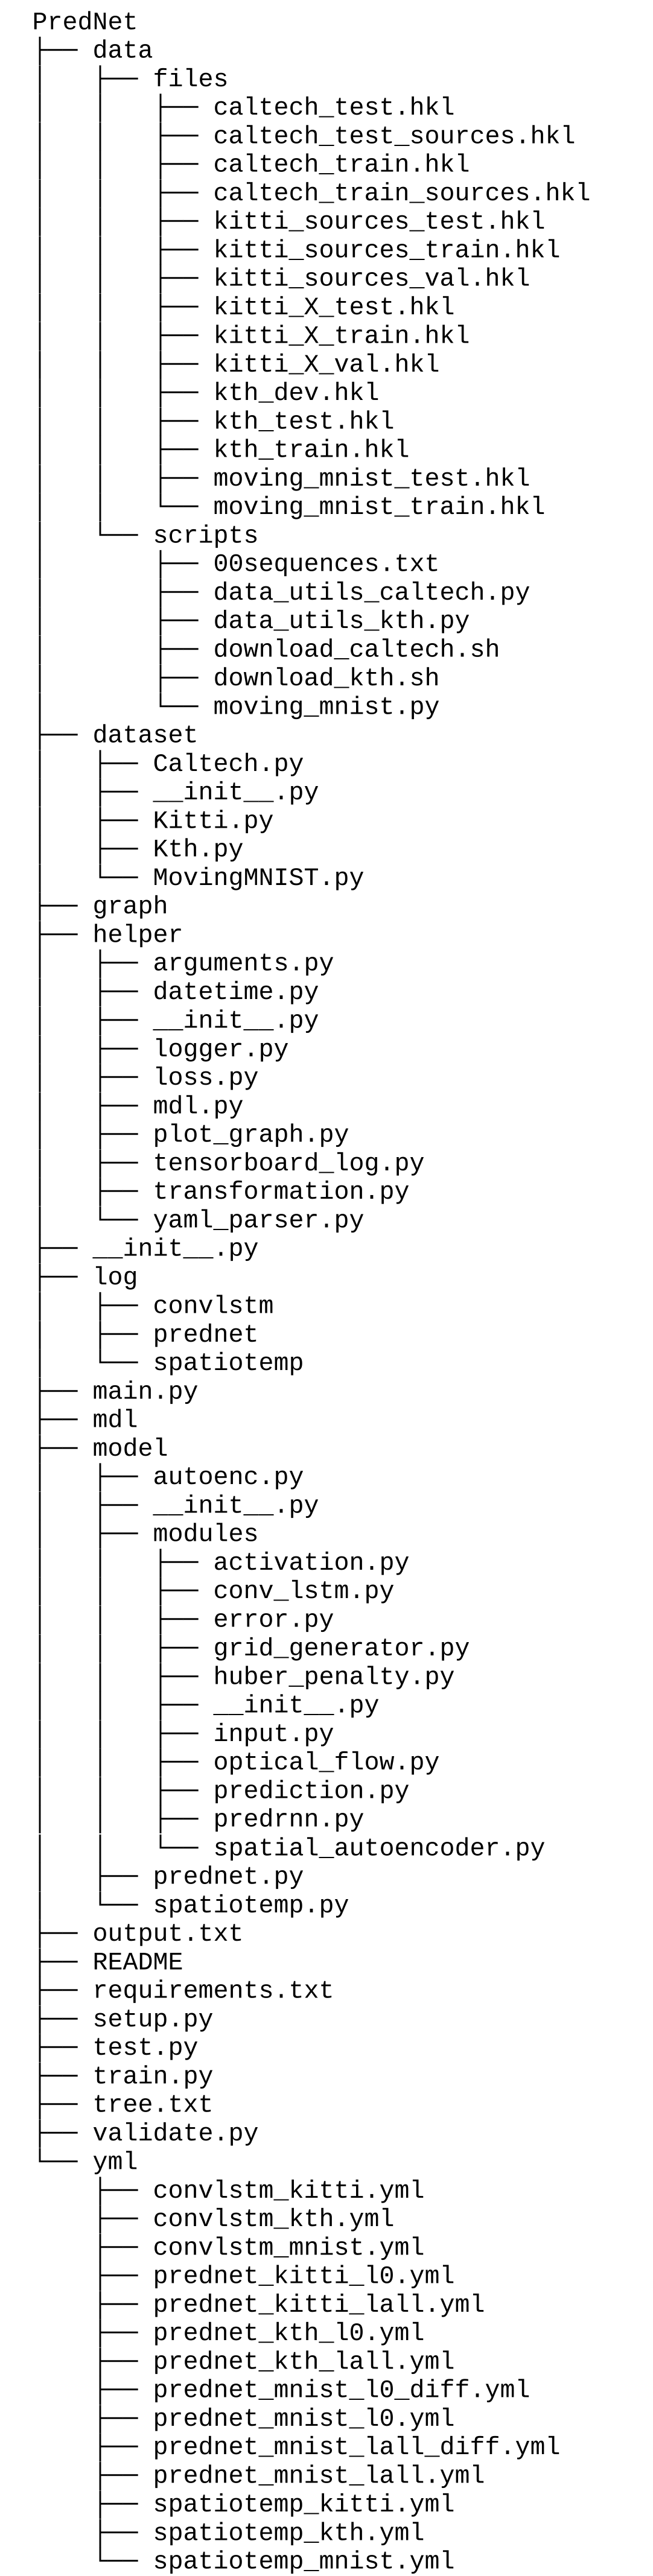
\includegraphics[width=0.3\textwidth]{../Images/tree.png}
   \centering
   \caption{Tree of Implementation}
   \label{fig:tree}
  \end{figure}\noindent
 % subsection
 \subsection*{Code usage}
  \begin{figure}[H]
   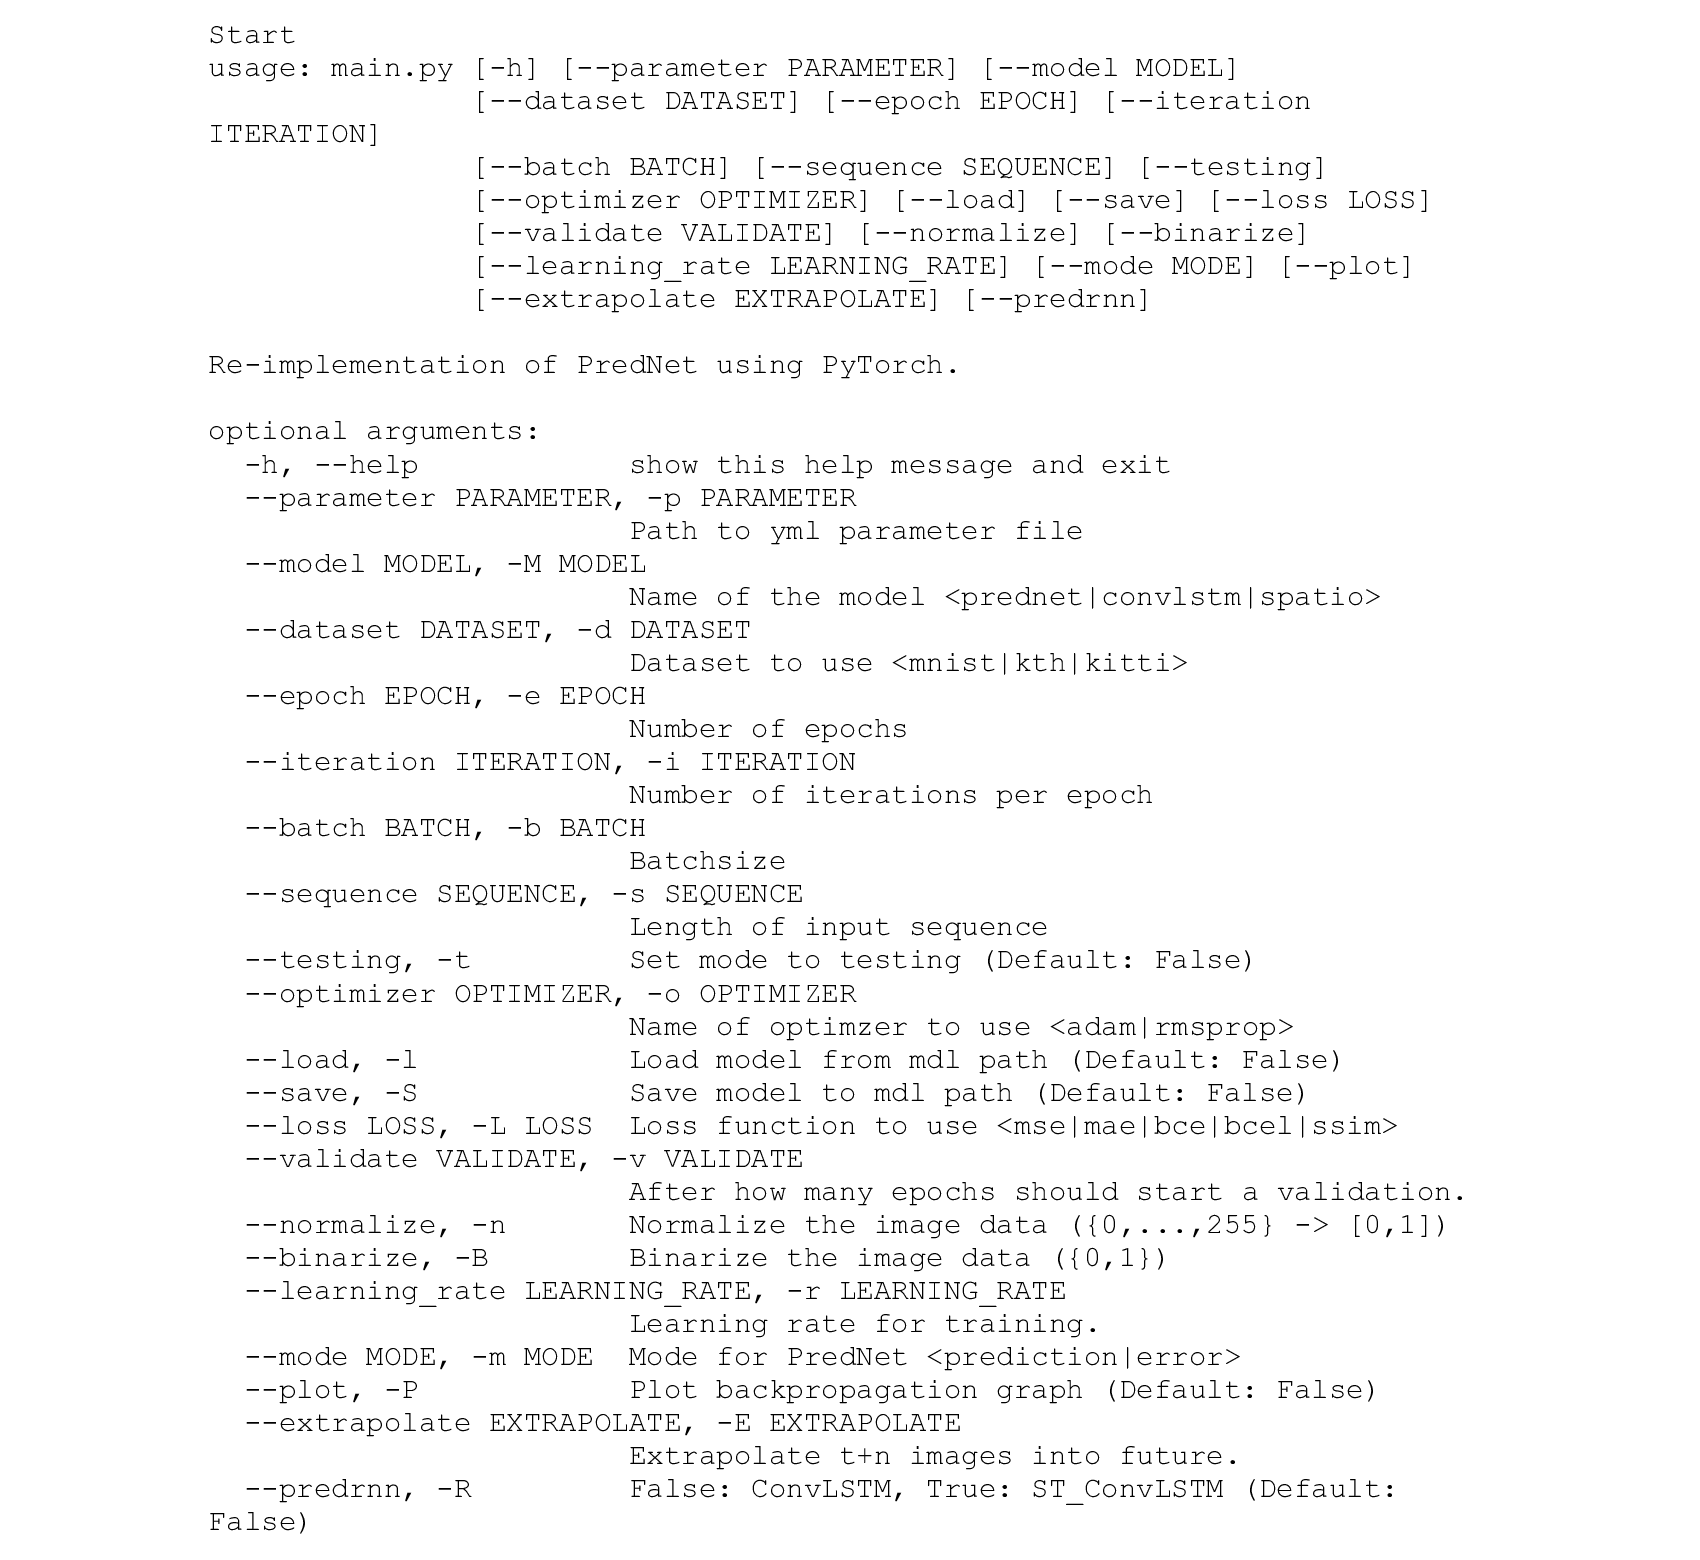
\includegraphics[width=1.0\textwidth]{../Images/usage.png}
   \centering
   \caption{Usage of Implementation}
   \label{fig:tree}
  \end{figure}\noindent
 \newpage

 % subsection
 \subsection*{Class diagram}
  \begin{figure}[H]
   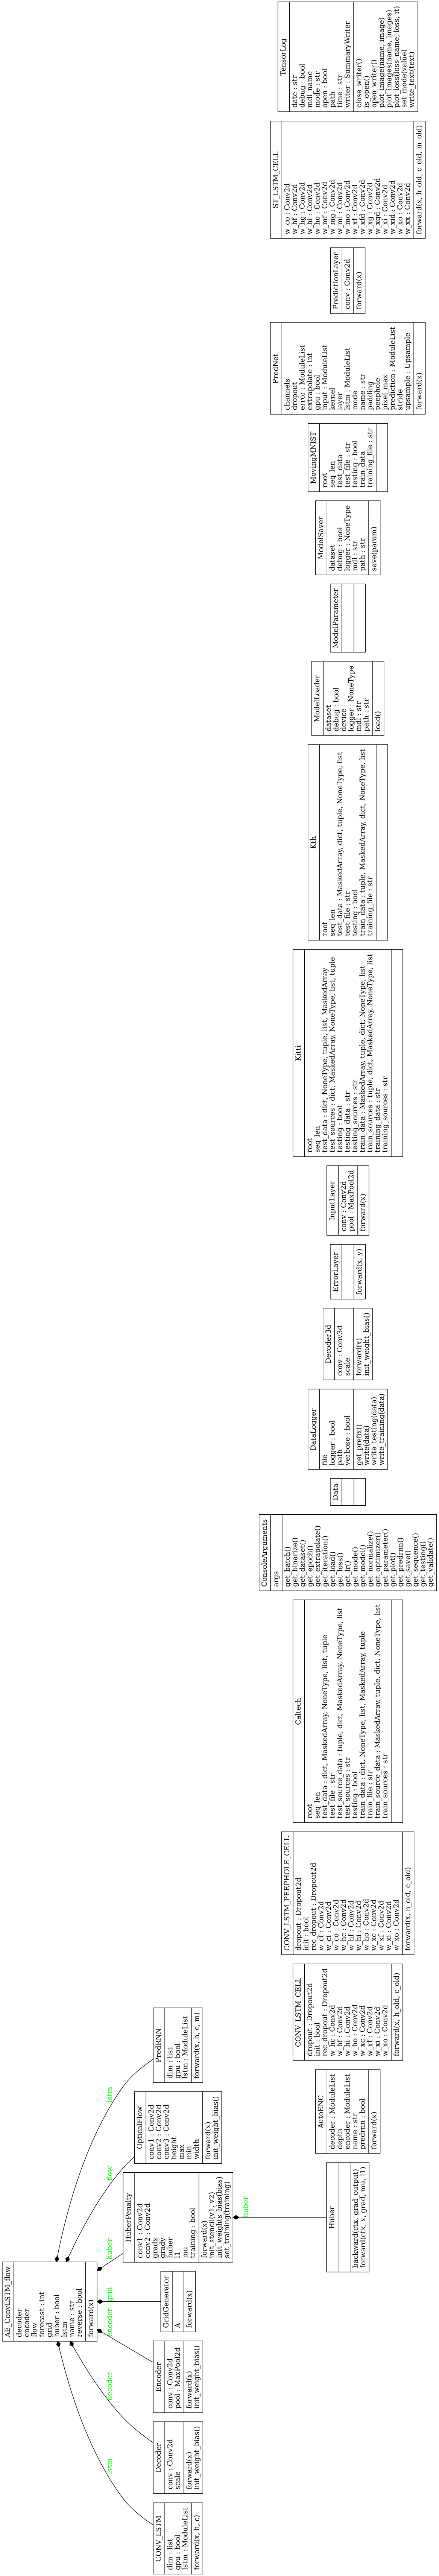
\includegraphics[width=0.23\textwidth]{../Images/classdiagram.png}
   \centering
   \caption{Class diagram, automatically provided by \href{https://pypi.org/project/pyreverse/}{pyreverse}. (pyreverse is not able find connections if loops are 
   used.)}
   \label{fig:tree}
  \end{figure}\noindent

 % subsection
 \subsection*{Package diagram}
  \begin{figure}[H]
   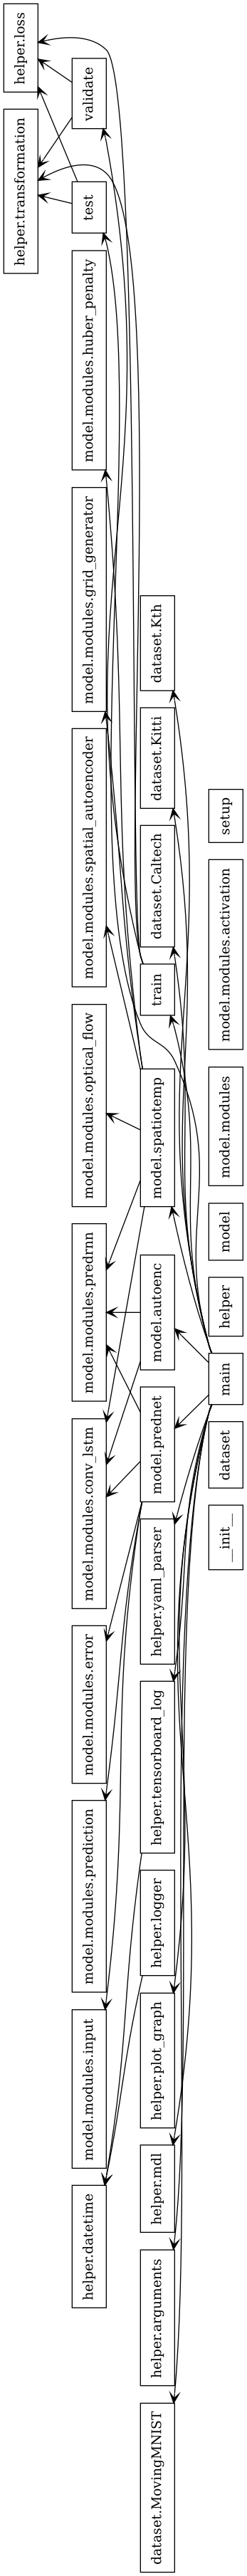
\includegraphics[width=0.13\textwidth]{../Images/packagediagram.png}
   \centering
   \caption{Package diagram, automatically provided by \href{https://pypi.org/project/pyreverse/}{pyreverse}}
   \label{fig:tree}
  \end{figure}\noindent

 % subsection  
 \subsection*{Experiments}
  \begin{center}
  \begin{turn}{90}
   \begin{tikzpicture}[font=\small, edge from parent fork down, level distance=1.75cm,
   every node/.style=
    {top color=white,
    bottom color=blue!25,
    rectangle,rounded corners,
    minimum height=8mm,
    draw=blue!75,
    very thick,
    drop shadow,
    align=center,
    text depth = 0pt
    },
	edge from parent/.style=
    {draw=blue!50,
    thick
    }]
	\Tree [.Experiments
        [.{Autoencoder}
            [.{ConvLSTM}
            	[.{MNIST} ]
            	[.{KTH} ]
            	[.{Kitti} ] ]
            [.{PredRNN}
            	[.{MNIST} ]
            	[.{KTH} ]
            	[.{Kitti} ] ] ] 
        [.{PredNet}
            [.{ConvLSTM}
            	[.{MNIST} ]
            	[.{KTH} ]
            	[.{Kitti} ] ]
            [.{PredRNN}
            	[.{MNIST} ]
            	[.{KTH} ]
            	[.{Kitti} ] ] ] 
        [.{Spatiotemp}
		    [.{ConvLSTM}
            	[.{MNIST} ]
            	[.{KTH} ]
            	[.{Kitti} ] ]
            [.{PredRNN}
            	[.{MNIST} ]
            	[.{KTH} ]
            	[.{Kitti} ] ] ] 
]
\end{tikzpicture}  
  \end{turn}
  \end{center}
  
 % subsection
 \subsection*{Experimental Results}
  % subsubsection
  \subsubsection*{MovingMNIST}
   \begin{figure}[H]
   \centering
   \subfloat[Ground truth]{{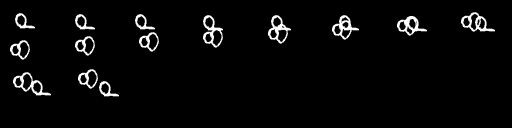
\includegraphics[width=0.85\textwidth]{../Images/convlstm_mnist_groundtruth.png} }} 
   \qquad
   \subfloat[ConvLSTM]{{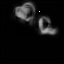
\includegraphics[width=0.1\textwidth]{../Images/convlstm_mnist_convlstm.png} }} 
   \qquad
   \subfloat[PredRNN]{{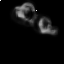
\includegraphics[width=0.1\textwidth]{../Images/convlstm_mnist_predrnn.png} }}
   \caption{Test results for Autoencoder on MovingMNIST.}
   \label{figure::convlstm_mnist_results}
   \end{figure}\noindent
   \begin{figure}[H]
   \centering
   \subfloat[Ground truth]{{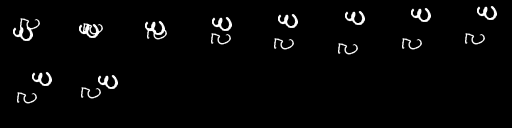
\includegraphics[width=0.85\textwidth]{../Images/spatiotemp_mnist_groundtruth.png} }} 
   \qquad
   \subfloat[ConvLSTM]{{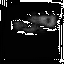
\includegraphics[width=0.1\textwidth]{../Images/spatiotemp_mnist_convlstm.png} }} 
   \qquad
   \subfloat[PredRNN]{{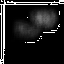
\includegraphics[width=0.1\textwidth]{../Images/spatiotemp_mnist_predrnn.png} }}
   \caption{Test results for Spatio-temporal Autoencoder on MovingMNIST.}
   \label{figure::spatiotemp_mnist_results}
   \end{figure}\noindent 
  
  % subsubsection
  \subsubsection*{KTH}
   \begin{figure}[H]
   \centering
   \subfloat[Ground truth]{{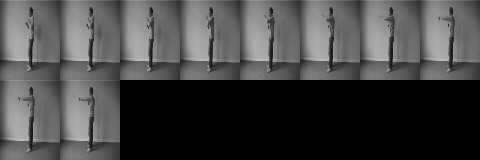
\includegraphics[width=0.85\textwidth]{../Images/convlstm_kth_groundtruth.png} }} 
   \qquad
   \subfloat[ConvLSTM]{{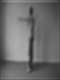
\includegraphics[width=0.1\textwidth]{../Images/convlstm_kth_convlstm.png} }} 
   \qquad
   \subfloat[PredRNN]{{
\includegraphics[width=0.1\textwidth]{../Images/convlstm_kth_predrnn.png} }}
   \caption{Test results for Autoencoder on KTH.}
   \label{figure::convlstm_kth_results}
   \end{figure}\noindent
   \begin{figure}[H]
   \centering
   \subfloat[Ground truth]{{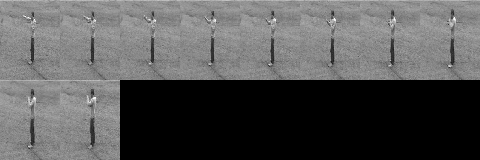
\includegraphics[width=0.85\textwidth]{../Images/spatiotemp_kth_groundtruth.png} }} 
   \qquad
   \subfloat[ConvLSTM]{{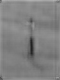
\includegraphics[width=0.1\textwidth]{../Images/spatiotemp_kth_convlstm.png} }} 
   \qquad
   \subfloat[PredRNN]{{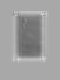
\includegraphics[width=0.1\textwidth]{../Images/spatiotemp_kth_predrnn.png} }}
   \caption{Test results for Spatio-temporal Autoencoder on KTH.}
   \label{figure::spatiotemp_kth_results}
   \end{figure}\noindent 
  
  % subsubsection
  \subsubsection*{Kitti}
   \begin{figure}[H]
   \centering
   \subfloat[Ground truth]{{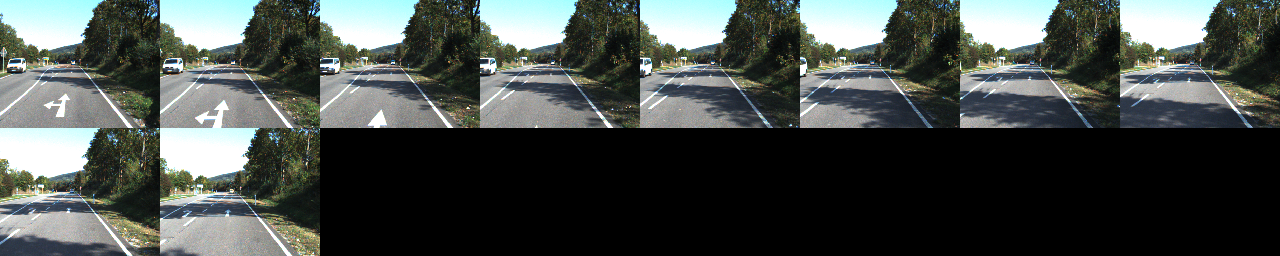
\includegraphics[width=1.0\textwidth]{../Images/convlstm_kitti_groundtruth.png} }} 
   \qquad
   \subfloat[ConvLSTM]{{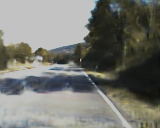
\includegraphics[width=0.15\textwidth]{../Images/convlstm_kitti_convlstm.png} }} 
   \qquad
   \subfloat[PredRNN]{{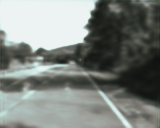
\includegraphics[width=0.15\textwidth]{../Images/convlstm_kitti_predrnn.png} }}
   \caption{Test results for Autoencoder on Kitti.}
   \label{figure::convlstm_kitti_results}
   \end{figure}\noindent
   \begin{figure}[H]
   \centering
   \subfloat[Ground truth]{{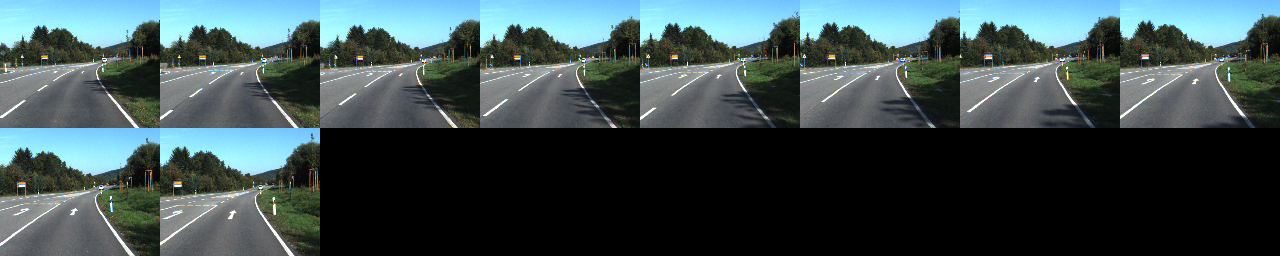
\includegraphics[width=1.0\textwidth]{../Images/spatiotemp_kitti_groundtruth.png} }} 
   \qquad
   \subfloat[ConvLSTM]{{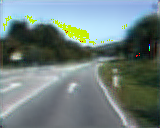
\includegraphics[width=0.15\textwidth]{../Images/spatiotemp_kitti_convlstm.png} }} 
   \qquad
   \subfloat[PredRNN]{{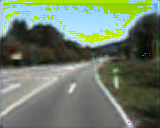
\includegraphics[width=0.15\textwidth]{../Images/spatiotemp_kitti_predrnn.png} }}
   \caption{Test results for Spatio-temporal Autoencoder on Kitti.}
   \label{figure::spatiotemp_kitti_results}
   \end{figure}\noindent 

 % subsection
 \subsection*{Backpropagation graphs}
  \begin{figure}[H]
   \includegraphics[width=1.0\textwidth]{../Images/convlstm_backgraph.png}
   \centering
   \caption{Backpropagation graph Autoencoder}
   \label{fig:backprop_autoenc}
  \end{figure}\noindent
  \begin{figure}[H]
   \includegraphics[width=1.0\textwidth]{../Images/prednet_backgraph.png}
   \centering
   \caption{Backpropagation graph PredNet}
   \label{fig:backprop_prednet}
  \end{figure}\noindent
  \begin{figure}[H]
   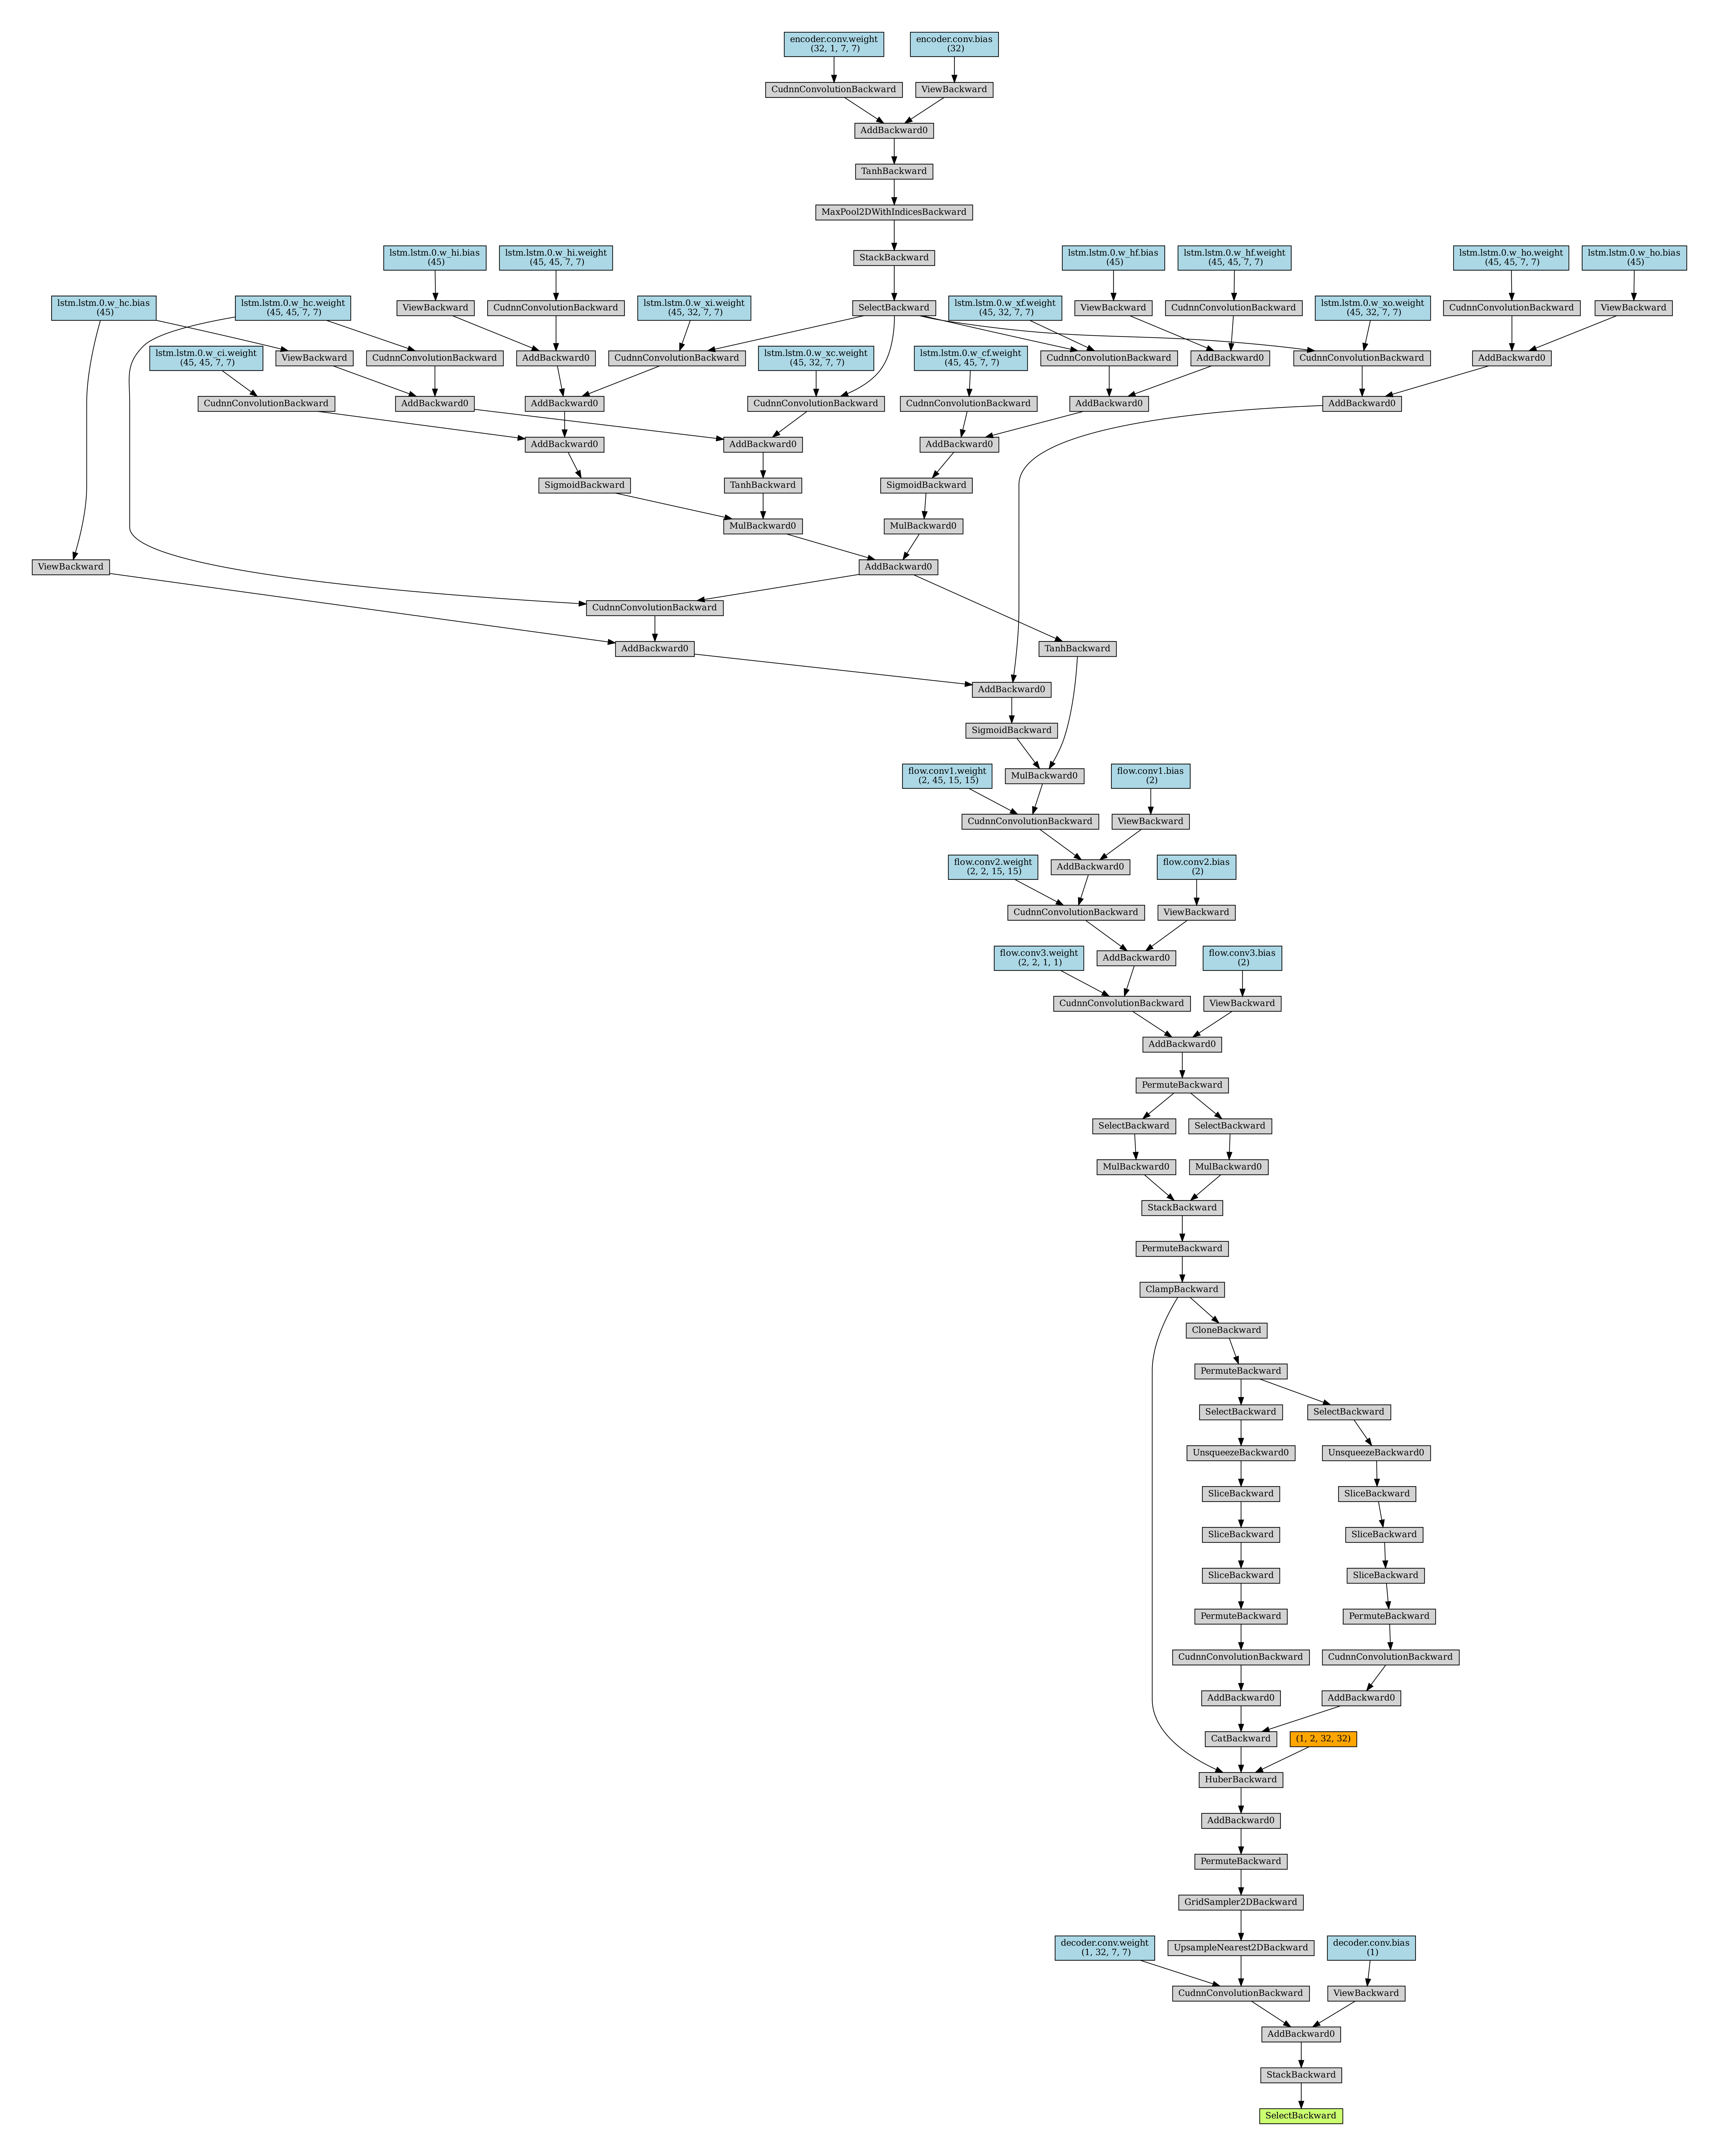
\includegraphics[width=1.0\textwidth]{../Images/spatiotemp_backgraph.png}
   \centering
   \caption{Backpropagation graph Spatiotemp}
   \label{fig:backprop_spatio}
  \end{figure}\noindent